\documentclass[a4paper]{article}
\usepackage[utf8]{inputenc}
\usepackage[english]{babel}
\usepackage{moreverb}
\usepackage{graphicx}
\usepackage{fancyvrb}
\title{Project Report \\ EDA216 Database Technology \\ Krusty Kookies AB}
\date{\today}
\author{Fredrik Paulsson \\ dat11fp1@student.lu.se \and Jonas Jacobsson \\ dat11jja@student.lu.se}
%\setcounter{secnumdepth}{5}
%\setcounter{tocdepth}{5}
\begin{document}
\maketitle
%\tableofcontents
\newpage

%Report
%The report should be written in English (you may write in Swedish if you absolutely cannot produce readable English). Contents:
%2
%1. A cover sheet with the name of the project, your names, education programs, and e-mail addresses. You must check mail to these addresses regularly.
%Also give the date of submission and complete instructions for running your program.
%2. An introduction (what the project is about, etc.).
%3. Something about requirements that you fulfill or don’t fulfill.
%4. An outline of your system (which database manager you use, which programs you have
%written, how the programs communicate with the database, etc.).
%5. An E/R diagram which describes the system.
%6. Relations. Indicate primary keys, possibly secondary keys, and foreign keys. You must
%show that the relations are normalized according to your chosen normal form (if a relation “obviously” is in BCNF you may say so, provided that you justify your statement). If a
%relation is in a lower normal form than BCNF, you must justify this choice.
%7. SQL statements to create all tables, views, stored procedures, and other database elements.
%(Don’t include statements to create the initial contents of the database.)
%8. A user’s manual (not necessary if everything in the program is self-explanatory).

\section{Introduction}
In this project we were to develop a database system that handles production, orders and deliveries of cookies in the company Krusty Kookies Sweden AB. In order to develop the database system we have to produce an E/R model of the database, create relations corresponding to the E/R model and finally implement those relations in a database management system. In the project we also had to implement a client program that interfaces to our database. This client program only handles production of cookies and blocking of pallets.

This report serves as documentation of our implementation. 

\section{Requirements}
Our database system can handle everything from ingrediences in the receipes to delivery of the cookies. 

The pallets are registered in our database when entering the freezer. To identify every pallet each pallet has a unique ID. We can list the pallets and information about each pallet. The receipe of the cookies, when it is made, if it is in the freezer and if it is block. If the pallet it is blocked the cookies do not meet the quality standards and can not be delivered.

When a new pallet is created the stock of the ingredients to make the receipe are updated to make sure the quantities of the ingredients in stock are correct. It is possible to check the amount of a ingredient in stock if needed.
%(We can not view the amount of ingredients which where delivered) 
% You are not able to change and add new receipes to our solution.
%
% Det har vi glömt.
%
% Visa info vid sökning: the contents of the pallet, the location of the pallet, if the pallet is delivered and in that case to whom, etc.
% Behövs delivered pallets och order då...och utvidgad select i findPallet($palledId).
%

\section{System Outline}
Our system uses MySQL as the database management system and our client interface is written in PHP for optimal portability. In PHP we have used PHP Data Object to interface with the MySQL server.


More specific to the client interface, our program can create an order of a wanted receipe and an amount of pallets with the cookies made from the receipe. If a batch of cookies do not meet the quality standards, you are able to block the pallets that are affected. Either through the pallet id or through the receipe and the time which the batch was made. 

\begin{description}
\item{}
\end{description}
\section{E/R Model}
\begin{figure}[!h]
\centering
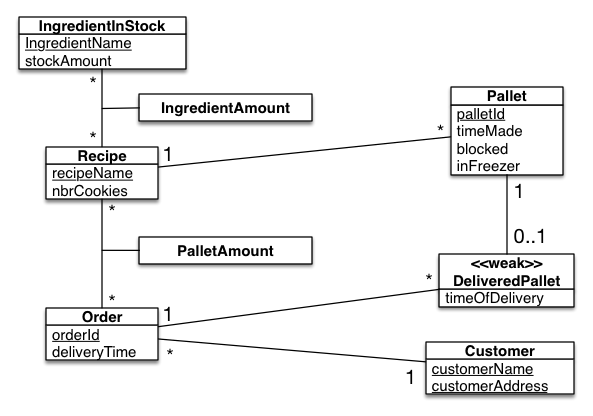
\includegraphics[scale=0.7]{projectUMLFinal.png}
\caption{UML diagram for the E/R model.}
\label{uml}
\end{figure}

\section{Relations}

\texttt{IngredientsInStock(\underline{ingredientName},stockAmount)} \\
\texttt{Recipes(\underline{recipeName},nbrCookies)} \\
\texttt{IngredientsInRecipe(\underline{\textit{ingredientName},\textit{recipeName}},ingredientAmount)} \\
\texttt{Customers(\underline{customerName,customerAddress})} \\
\texttt{Orders(\underline{orderId},deliveryTime,\textit{customerName,customerAddress})} \\
\texttt{RecipesInOrders(\underline{\textit{recipeName},\textit{orderId}},palletAmount)} \\
\texttt{Pallets(\underline{palletId},timeMade,blocked,inFreezer,\textit{recipeName})} \\
\texttt{DeliveredPallets(\underline{\textit{palletId}},timeOfDelivery,\textit{orderId})}

In these relations undelrined attributes are keys and attributes written in italics are foreign keys.

There exist no nontrivial functional dependencies except the ones whose left hand sides are the keys for each relation. Thus there exist no functional dependency that can break the BCNF condition.

\section{SQL Statements}
The following SQL statements have been issued to the MySQL DBMS in order to create our database.
\begin{Verbatim}
create table IngredientsInStock (
	ingredientName varchar(30),
	stockAmount integer,
	primary key (ingredientName)
);
create table Recipes (
	recipeName varchar(30),
	nbrCookies integer,
	primary key (recipeName)
);
create table IngredientsInRecipes (
	ingredientName varchar(30),
	recipeName varchar(30),
	ingredientAmount integer,
	primary key (ingredientName,recipeName),
	foreign key (ingredientName) references 
		IngredientsInStock(ingredientName),
	foreign key (recipeName) references Recipes(recipeName)
);
create table Customers (
	customerName varchar(40),
	customerAddress varchar(40),
	primary key (customerName,customerAddress)
);
create table Orders (
	orderId integer auto_increment,
	deliveryTime timestamp default current_timestamp,
	customerName varchar(40),
	customerAddress varchar(40),
	primary key (orderId),
	foreign key (customerName,customerAddress) references 
		Customers(customerName,customerAddress)
);
create table RecipesInOrders (
	recipeName varchar(30),
	orderId integer,
	palletAomunt integer,
	primary key (recipeName,orderId),
	foreign key (recipeName) references Recipes(recipeName),
	foreign key (orderId) references Orders(orderId)
);
create table Pallets (
	palletId integer auto_increment,
	timeMade timestamp default current_timestamp,
	blocked boolean,
	inFreezer boolean,
	recipeName varchar(30),
	primary key (palletId),
	foreign key (recipeName) references Recipes(recipeName)
);
create table DeliveredPallets (
	palletId integer,
	timeOfDelivery timestamp default current_timestamp,
	orderId integer,
	primary key (palletId),
	foreign key (palletId) references Pallets(palletId),
	foreign key (orderId) references Orders(orderId)
);
\end{Verbatim}

\section{User Manual}
%\begin{thebibliography}{1}
%\bibitem{wikipedia}
%http://en.wikipedia.org
%\end{thebibliography}
\end{document}